\chapter{从动量模式到局域量子场}

什么是量子场，它与粒子有何关系？基本的数学工具是谐振子。一个场包含许多可能的振荡模式，而场的量子化就相当于为每个模式各配上一个量子谐振子。这一构造最容易先在有限周期空间中看出，在那里允许的模式构成一个离散的列表。

\section{周期空间与允许的波数}

取一个空间坐标\(x\)，并把相距\(L\)的点等同起来。可以把该空间想象成周长为\(L\)的圆。这是一个有用的有限体积技巧。在带端点的有限区间上，行波会从端点反射。在周期区间上，它可以沿任一方向继续传播而不反射。平移对称性、因而动量守恒得以保留，同时无限体积带来的复杂性被暂时消除。

平面波具有形式
\begin{equation}
e^{ikx}.
\end{equation}
绕圆一周之后，它必须回到原来的值。由于波在\(x=0\)处等于\(1\)，周期性要求
\begin{equation}
e^{ikL}=1.
\end{equation}
为什么\(2\pi\)的整数倍能满足这一条件？欧拉公式给出
\begin{align}
e^{i2\pi n}
&=\cos(2\pi n)+i\sin(2\pi n)\\
&=1,
\qquad n\in\mathbb Z.
\end{align}
经过任意整数个周期后，余弦为\(1\)，正弦为\(0\)。因此，
\begin{equation}
kL=2\pi n,
\qquad
k=\frac{2\pi n}{L},
\qquad n\in\mathbb Z.
\end{equation}
量\(k\)是波数。整数\(n\)标记一个允许的波数；它还不是在计数粒子。

同一条件也可以用波长来表示。波长是相位前进整整一个周期的距离，因此
\begin{equation}
k\lambda=2\pi,
\qquad
k=\frac{2\pi}{\lambda}.
\end{equation}
长波长对应小波数，短波长对应大波数。周期性条件说的是，整数个波长恰好绕圆一周。

对于量子力学波，动量为
\begin{equation}
p=\frac{h}{\lambda}
=\frac{2\pi\hbar}{\lambda}
=\hbar k.
\end{equation}
因此\(k\)与\(p\)只相差因子\(\hbar\)。正的和负的\(k\)描述沿相反方向运动的波以及动量方向相反的粒子。在\(\hbar=1\)的单位制下，通常就把\(k\)称为动量，不再作进一步区分。

对于每一个允许的\(k\)，该模式中可以有若干个量子。这引入了第二个整数：
\begin{equation}
n(k)=\text{number of quanta with wave number }k.
\end{equation}
它称为占据数。\(k=2\pi n/L\)中的整数标记模式；\(n(k)\)则表明有多少粒子占据该模式。无论\(k\)为正还是为负，都必须给出占据数。

\begin{classroomqa}
\lecturetimestamp{00:11:58}
\audiencequestion{\(k\)本身是整数吗？}
\lecturerresponse{不是。波数是\(2\pi/L\)的整数倍：\(k=2\pi n/L\)。该公式中的整数\(n\)标记允许的动量，它与占据数\(n(k)\)不同，后者计数该模式中的量子。}
\end{classroomqa}

\section{占据数态与模式算符}

量子态是一个矢量，或线性元素。态矢量可以相加，也可以乘以数，而算符作用于它们会产生其他态矢量。可观测的实数量由厄米算符表示。这些基本事实在这里很重要，因为多粒子态和场都将由线性组合与算符构造出来。

令
\begin{equation}
k_j=\frac{2\pi j}{L},
\qquad j\in\mathbb Z.
\end{equation}
多粒子态的一个方便标记就是整串占据数。用简写\(n_j\equiv n(k_j)\)表示所显示的各个条目，写出
\begin{equation}
\big|\{n(k_j)\}\big\rangle
=
\big|\ldots,n_{-2},n_{-1},n_0,n_1,n_2,\ldots\big\rangle.
\end{equation}
条目\(n(k_1)\)是第一个正动量模式中的粒子数，\(n(k_2)\)是第二个模式中的粒子数，依此类推。这串数向两个方向无限延伸。

\begin{figure}[t]
\centering
\includegraphics[width=0.72\textwidth]{lecture_03_figure_02.png}
\caption{允许动量模式的占据数\(n(k)\)。}
\lectureframe{00:15:04}
\end{figure}

每个动量模式都是一个谐振子。因此它有一个升算符和一个降算符。最初写作\(a^{+}(k)\)和\(a^{-}(k)\)的记号，将写作\(a^\dagger(k)\)和\(a(k)\)。它们的作用为
\begin{align}
a^\dagger(k)\big|\ldots,n(k),\ldots\big\rangle
&=
\sqrt{n(k)+1}\notag\\
&\quad{}\times
\big|\ldots,n(k)+1,\ldots\big\rangle,
\\
a(k)\big|\ldots,n(k),\ldots\big\rangle
&=
\sqrt{n(k)}\,
\big|\ldots,n(k)-1,\ldots\big\rangle.
\end{align}
算符\(a^\dagger(k)\)作用于属于\(k\)的槽位，把该占据数升高一，并把态乘以\(\sqrt{n(k)+1}\)。算符\(a(k)\)降低同一个槽位，并给出\(\sqrt{n(k)}\)。每一个允许的动量都有一个这样的算符对。

\begin{figure}[t]
\centering
\includegraphics[width=0.58\textwidth]{lecture_03_figure_03.png}
\caption{与动量模式\(k\)相联系的产生算符和湮灭算符。}
\lectureframe{00:17:14}
\end{figure}

\section{傅里叶系数成为算符}

这些振子算符与场之间的联系，始于一个普通的经典傅里叶级数。周期区间上的复经典场可以写成
\begin{align}
\psi(x)&=\sum_k \alpha(k)e^{ikx},\\
\psi^*(x)&=\sum_k \alpha^*(k)e^{-ikx},
\end{align}
其中每个求和都遍历允许的取值 \(k=2\pi n/L\)。这等价于把场按正弦和余弦展开。

复场有实部和虚部。它的复共轭使虚部变号，\(e^{ikx}\) 变为 \(e^{-ikx}\)。指定所有系数 \(\alpha(k)\) 就指定了经典场。一旦 \(\alpha(k)\) 已知，就不必再独立指定 \(\alpha^*(k)\)，但每个系数的实部和虚部是各自独立的实数量。它们可以作为相应傅里叶分量的振幅被测量。在这个意义上，一个复系数打包了两个经典可观测量。

量子化把这些经典傅里叶系数替换为算符。普通的等号会把不同种类的对象等同起来，所以最好写成一个替换规则：
\begin{equation}
\alpha(k)\rightsquigarrow a(k),
\qquad
\alpha^*(k)\rightsquigarrow a^\dagger(k).
\end{equation}
在傅里叶符号取法一致的情况下，量子场由下式定义
\begin{align}
\Psi(x)&=\sum_k a(k)e^{ikx},\\
\Psi^\dagger(x)&=\sum_k a^\dagger(k)e^{-ikx}.
\end{align}
\editorialnote{口头讨论改变了傅里叶符号约定，后来又对其提出质疑。这里所用的共轭对，是在更清晰的场展开和位置态计算中可见的约定：\(\Psi\) 携带 \(e^{ikx}\)，而 \(\Psi^\dagger\) 携带 \(e^{-ikx}\)。把所有符号一致地反过来，会描述同样的构造。}

目前，这只是一个定义：量子场是系数为算符的傅里叶和。更充分的论证必须表明，这些算符如何在适当的极限下重现经典系数，而这需要一些动力学。那个问题被推迟了。已经清楚的是，场本身是一个算符，而它的傅里叶系数之间的关系就是谐振子的产生与湮灭关系。

\begin{classroomqa}
\lecturetimestamp{00:26:48}
\audiencequestion{引入产生和湮灭算符，是否意味着动力学必然产生和消灭粒子？}
\lecturerresponse{不。这些算符是改变占据数的数学操作。自然规律是否真的改变粒子数，是一个关于动力学的问题。如果动力学允许这种改变，这些算符就为描述它们提供了自然的语言。}
\end{classroomqa}

\section{散射与粒子数可变}

首先考虑一个不改变粒子数的过程。假设最初唯一存在的粒子具有动量 \(k_7\)。在占据数记号中，它的状态在第七个位置有一个 \(1\)，其余各处都是零：
\begin{equation}
|k_7\rangle
=
|\ldots,0,\underset{k_7}{1},0,\ldots\rangle.
\end{equation}
一个散射过程把它的动量从 \(k_7\) 改变为 \(k_9\)。恰好实现这一改变的算符是
\begin{equation}
a^\dagger(k_9)a(k_7).
\end{equation}
最右边的算符先作用：它移除 \(k_7\) 位置上的粒子。然后左边的算符在 \(k_9\) 位置上产生一个粒子。

\begin{classroomqa}
\lecturetimestamp{00:31:37}
\audiencequestion{在这个 \(k_7\to k_9\) 过程中，平方根因子从哪里进入？}
\lecturerresponse{湮灭因子是 \(\sqrt{n(k_7)}=\sqrt{1}=1\)。在这次移除之后，系统处于全零态。由于 \(k_9\) 模是空的，产生因子是 \(\sqrt{n(k_9)+1}=\sqrt{1}=1\)。因此，在这个单粒子例子中，两个因子都不改变数值系数。}
\end{classroomqa}

让我们执行这两个步骤。湮灭给出
\begin{align}
a(k_7)|k_7\rangle
&=
\sqrt{1}\,|\ldots,0,0,0,\ldots\rangle\\
&=|0\rangle.
\end{align}
全零态就是真空。它是没有粒子的状态，而在这个简单的振子集合中，它也是基态。接着在空的 \(k_9\) 模中产生给出
\begin{equation}
a^\dagger(k_9)|0\rangle
=\sqrt{0+1}\,|k_9\rangle
=|k_9\rangle.
\end{equation}
因此，
\begin{equation}
a^\dagger(k_9)a(k_7)|k_7\rangle=|k_9\rangle.
\end{equation}
逐个位置看，唯一的 \(1\) 只是从第七个动量模移到了第九个。由于占据数从未超过一，两个平方根因子都等于一。一旦涉及一个已被占据的模，它们就会变得重要。

这个一对一的过程也可以用普通的单粒子量子力学来描述：一个粒子改变其动量。当粒子数可以改变时，占据数语言就变得不可或缺。例如，
\begin{equation}
a^\dagger(k_9)a^\dagger(k_{16})a(k_7)|k_7\rangle
=|k_9,k_{16}\rangle
\end{equation}
描述从模 \(k_7\) 中的一个入射粒子到两个出射粒子（一个在 \(k_9\)，一个在 \(k_{16}\)）的数学改变。一个靶可以吸收入射粒子，发射两个出射粒子，并承担所需的任何反冲。这样的过程无法在限制于一个粒子的希尔伯特空间中表示，但它自然地适合一个占据数可以变化的状态空间。算符表达式本身并不是自然规律；它是用来书写一条改变粒子数的规律的语言。

\section{点上的场算符}

位置空间算符\(\Psi^\dagger(x)\)产生什么？量子态构成线性空间：动量态可以用复系数相加，形成新的态。从真空出发。由于每个模式都是空的，
\begin{equation}
\Psi(x)|0\rangle=0.
\end{equation}
右边的零是零矢量：湮灭算符找不到任何粒子可以移除。

共轭场的作用不同：
\begin{align}
\Psi^\dagger(x)|0\rangle
&=\sum_k e^{-ikx}a^\dagger(k)|0\rangle\\
&=\sum_k e^{-ikx}|k\rangle,
\end{align}
其中
\begin{equation}
|k\rangle=a^\dagger(k)|0\rangle
\end{equation}
是动量为\(\hbar k\)的单粒子态。

\begin{figure}[t]
\centering
\includegraphics[width=0.70\textwidth]{lecture_03_figure_05.png}
\caption{形式上的位置空间态\(\Psi^\dagger(x)|0\rangle\)按单粒子动量态展开。}
\lectureframe{00:43:16}
\end{figure}

在形式上，并且不计归一化，这个求和就是单粒子量子力学中的广义位置态。\footnote{由于动量模式有无穷多个，严格局域的位置态是不可归一化的。若引入有限的动量截断，并对截断后的求和进行归一化，则得到一个以\(x\)为中心的、高度局域的波包。}动量本征态与系数\(e^{-ikx}\)组合，产生在\(x\)处的局域化。在这种形式意义上，
\begin{equation}
\Psi^\dagger(x)\ \text{creates a particle at position }x,
\end{equation}
而
\begin{equation}
\Psi(x)\ \text{annihilates a particle at position }x.
\end{equation}
模式算符\(a^\dagger(k)\)产生具有确定动量的粒子。场算符\(\Psi^\dagger(x)\)产生允许动量态的相干叠加，该叠加在形式上局域于\(x\)。

在形式上的未归一化求和中，每个系数\(e^{-ikx}\)的模都为1。在有限截断下，归一化后的截断态对保留下来的动量具有等模系数，而它们的相位产生一个在\(x\)附近高度局域的波包。这就是量子场与粒子之间的基本联系。

暂时忽略狭义相对论的复杂性，在这个模型中\(\Psi^\dagger(x)\)在\(x\)处产生一个粒子。相对论性场需要进一步修正，但算符值的傅里叶展开以及动量模式算符与位置空间算符之间的区别仍然是基本的。

\begin{classroomqa}
\lecturetimestamp{00:44:59}
\audiencequestion{\(x\)是周期圆上的一个点吗？当圆变大时会发生什么？}
\lecturerresponse{是的。在有限模型中，\(x\)是圆上的一个点。相邻的允许波数之间相隔\(2\pi/L\)。随着\(L\)增大，这个间距变小，因此对于每一个想要的动量，都有一个任意接近它的允许值。在无限体积极限下，对\(k\)的求和被对\(k\)的积分取代。先理解离散求和是有用的。}
\end{classroomqa}

\section{局域粒子反应}

一旦\(\Psi(x)\)和\(\Psi^\dagger(x)\)被解释为在一点上湮灭和产生粒子，局域性就可以直接表达。设想一个粒子被一个锐局域于\(x\)处的靶吸收，而一个出射粒子突然出现在半人马座{\proseunicodefont α}附近，另一个出现在参宿四附近。这样的反应是非局域的：其分离的事件无法通过普通传播联系起来。

人们可以先放宽要求，允许出射粒子在靶周围一个小区域内的某处发射。精确的局域理想化更强：如果入射粒子在\(x\)处被吸收，那么出射粒子就在同一点产生。使用在分离点上求值的场则会描述一个非局域的算符乘积。因此，局域的一变二操作是
\begin{equation}
\Psi^\dagger(x)\Psi^\dagger(x)\Psi(x).
\end{equation}
最右边的场在\(x\)处移除入射粒子；它左边的两个场在那里产生两个出射粒子。\footnote{局域的一变二示意图遵循在00处描述的反应：47:38--00:49:13。}

\begin{figure}[t]
\centering
\begin{tikzpicture}[scale=1.0]
\draw[->] (-2.2,0) -- (0,0);
\fill (0,0) circle (2.2pt);
\draw[->] (0,0) -- (2.0,1.1);
\draw[->] (0,0) -- (2.0,-1.1);
\node at (-1.25,0.3) {$k_{\mathrm{initial}}$};
\node[right] at (0.05,0.05) {$x$};
\node at (1.48,1.34) {$\ell$};
\node at (1.48,-1.34) {$m$};
\end{tikzpicture}
\caption{一个入射粒子在\(x\)处被吸收，两个出射粒子在同一点产生。}
\end{figure}

设入射态包含一个具有确定波数\(k_{\mathrm{initial}}\)的粒子。为了确定出射动量，代入局域场的动量空间展开。把固定的动量标签与哑求和指标区分开来很重要。写出
\begin{align}
\Psi(x)&=\sum_q a(q)e^{iqx},\\
\Psi^\dagger(x)&=\sum_\ell a^\dagger(\ell)e^{-i\ell x}.
\end{align}
指标\(q\)被求和，而\(k_{\mathrm{initial}}\)标记特定的被占据入射模式。两个\(\Psi^\dagger(x)\)副本也需要独立的哑指标，比如\(\ell\)和\(m\)。重复使用一个指标会错误地把两个独立的求和绑在一起。这里\(\ell\)和\(m\)是波数；\(m\)不表示质量。

一个具体的图景是：一个光子撞击定域在\(x\)处的一个原子，随后两个光子从该点离开。这里所用的简单场更适合非相对论性粒子，而不太适合完全相对论性的光子场，因此光子的说法只是在说明算符的记账方式。

湮灭场先作用：
\begin{align}
\Psi(x)|k_{\mathrm{initial}}\rangle
&=\sum_q e^{iqx}a(q)a^\dagger(k_{\mathrm{initial}})|0\rangle.
\end{align}
除\(q=k_{\mathrm{initial}}\)的那一项外，每一项都为零。湮灭算符必须在其自身的模式中找到粒子。因此
\begin{equation}
\Psi(x)|k_{\mathrm{initial}}\rangle
=e^{ik_{\mathrm{initial}}x}|0\rangle.
\end{equation}
随后两个产生场给出
\begin{align}
&\Psi^\dagger(x)\Psi^\dagger(x)\Psi(x)
|k_{\mathrm{initial}}\rangle
\\
&\quad=
e^{ik_{\mathrm{initial}}x}
\sum_{\ell,m}
e^{-i\ell x}e^{-imx}
a^\dagger(\ell)a^\dagger(m)|0\rangle
\\
&\quad=
\sum_{\ell,m}
e^{i(k_{\mathrm{initial}}-\ell-m)x}
a^\dagger(\ell)a^\dagger(m)|0\rangle.
\end{align}
对于不相等的\(\ell\)和\(m\)，该算符态可记为\(|\ell,m\rangle\)：两个模式中各有一个粒子。最终结果是遍及所有这类双粒子动量位形的求和，其相位由入射和出射动量决定。

\begin{classroomqa}
\lecturetimestamp{01:00:36}
\audiencequestion{两个产生算符对易吗？}
\lecturerresponse{对易。所有产生算符彼此对易，所有湮灭算符也彼此对易。一个产生算符和一个湮灭算符在涉及不同模式时对易；对于同一模式，它们的对易子不为零。}
\end{classroomqa}

\begin{classroomqa}
\lecturetimestamp{01:01:34}
\audiencequestion{两个出射动量应当满足动量守恒吗？}
\lecturerresponse{所显示的粒子本身不必守恒动量，因为原子或靶可以反冲。差值\(k_{\mathrm{initial}}-\ell-m\)就是转移给靶的动量。包括靶在内的总动量才是守恒量。}
\end{classroomqa}

由于系数\(e^{i(k_{\mathrm{initial}}-\ell-m)x}\)是纯相位，其模为一。乍看之下，这暗示所有配对\((\ell,m)\)具有相同的概率权重。然而，当两个标记重合时，有一个重要的限定。

若\(\ell=m\)，则第一个产生算符把一个粒子放入模式\(m\)，而第二个作用于一个已被占据一次的模式：
\begin{align}
a^\dagger(m)a^\dagger(m)|0\rangle
&=a^\dagger(m)|1_m\rangle\\
&=\sqrt{2}\,|2_m\rangle.
\end{align}
因此，在同一模式中的双重产生具有一个额外的振幅\(\sqrt{2}\)。振幅平方后在概率中产生一个因子\(2\)。

\begin{classroomqa}
\lecturetimestamp{01:04:54}
\audiencequestion{因为产生系数含有\(n+1\)，\(\ell\)和\(m\)就必须相差一吗？}
\lecturerresponse{不是。符号\(\ell\)和\(m\)标记的是动量模式。\(\sqrt{n+1}\)中的\(n\)是产生算符所作用的那个特定模式的占据数。动量标记和粒子数是不同的整数。}
\end{classroomqa}

\begin{figure}[t]
\centering
\includegraphics[width=0.92\textwidth]{lecture_03_figure_06.png}
\caption{局域的一变二粒子振幅的动量空间展开。}
\lectureframe{01:05:44}
\end{figure}

这一构造中的粒子是全同的。因此\(\sqrt{2}\)是玻色子占据因子，而不是区分第一个粒子与第二个粒子的标记。将其平方，暂时看来会使同动量结果比单个不等动量项的概率大一倍。一旦仔细计数双重求和中的各项，这一比较还需要重新审视。

\begin{classroomqa}
\lecturetimestamp{01:06:43}
\audiencequestion{在一个复杂的反应中，产生算符和湮灭算符的次序是如何选定的？}
\lecturerresponse{所有产生算符在左、湮灭算符在右的表达式称为正规序。在这种形式中，最右边的算符先移除入射粒子，其余算符则产生出射粒子。}
\end{classroomqa}

重排一个混合的产生--湮灭对通常不是简单的置换：它必须使用对易子，而对于同一模式，这会产生一个额外项。\footnote{这一对易子限定是对01处非正式正规序讨论的编辑更正：06：43。}

\begin{classroomqa}
\lecturetimestamp{01:07:30}
\audiencequestion{如果所有动量振幅都具有相同的模，那么诸如``两倍概率''这样的说法是什么意思？}
\lecturerresponse{要记住有限腔体。其允许的动量是离散的，因此可以逐模式比较概率。这种比较不是在连续统中孤立点的概率之间进行的。}
\end{classroomqa}

对于\(\ell\ne m\)，无限制的双重求和包含两个有序项
\begin{equation}
a^\dagger(\ell)a^\dagger(m)|0\rangle
\quad\text{and}\quad
a^\dagger(m)a^\dagger(\ell)|0\rangle.
\end{equation}

\begin{classroomqa}
\lecturetimestamp{01:08:24}
\audiencequestion{当\(\ell\ne m\)时，同一末态在双重求和中会出现两次，一次作为\((\ell,m)\)，一次作为\((m,\ell)\)吗？}
\lecturerresponse{是的。若\(\ell\ne m\)，则项\((\ell,m)\)和\((m,\ell)\)都出现，并且由于产生算符对易，它们描述的是同一物理态。}
\end{classroomqa}

这两个有序项相等，因此在定量比较通道之前，必须先处理态归一化和这种重复计数。可靠的代数结论更窄，且足以支撑后续内容：在已被\(n\)个全同玻色子占据的模式中产生粒子，会给出因子\(\sqrt{n+1}\)。

\section{自发发射与受激发射}

一个更清晰的例子可以分离出平方根因子。假设一个定域在\(x\)处的物体发射一个光子。如果光子场初始处于真空态，则出射态为
\begin{align}
\Psi^\dagger(x)|0\rangle
&=\sum_k e^{-ikx}a^\dagger(k)|0\rangle\\
&=\sum_k e^{-ikx}|k\rangle.
\end{align}
在这个简化模型中，所有动量的振幅大小都相等。由于原本没有光子存在，这种发射是自发发射。

现在假设模式\(\ell\)中已经有一个光子。用同一个局域产生场作用，会给出两类项：
\begin{equation}
\Psi^\dagger(x)|\ell\rangle
=
\sum_{k\ne\ell}e^{-ikx}|k,\ell\rangle
+e^{-i\ell x}\sqrt{2}\,|2_\ell\rangle.
\end{equation}
对于\(k\ne\ell\)，算符产生到空模式中，因此系数为\(\sqrt{0+1}=1\)。对于\(k=\ell\)，算符产生到已被占据的模式中，因此系数为\(\sqrt{1+1}=\sqrt{2}\)。原来的光子是旁观者；新光子优先发射到它已占据的模式中。

\begin{classroomqa}
\lecturetimestamp{01:16:14}
\audiencequestion{预先存在的光子必须位于同一位置才能受激发射吗？}
\lecturerresponse{这个简化计算指的是同一动量模式的占据，而不是两个粒子位于同一个被精确确定的位置。一个粒子不可能同时具有精确的位置和精确的动量。真实光子由波包描述，而腔的理想化则给出确定的离散模式。在这种情形下，增强是进入已被占据的腔模式。}
\end{classroomqa}

如果模式\(\ell\)初始包含\(n_\ell\)个光子，那么
\begin{equation}
a^\dagger(\ell)
|\ldots,n_\ell,\ldots\rangle
=
\sqrt{n_\ell+1}
\,|\ldots,n_\ell+1,\ldots\rangle.
\end{equation}
因此概率被因子\(n_\ell+1\)增强。若已经存在一个光子，该因子为\(2\)。若该模式中有一百个光子，则振幅因子为\(\sqrt{101}\)，而发射到该模式的概率是空模式值的\(101\)倍。玻色子模式中已有的量子数越多，下一个量子就越可能发射到该模式中。这就是受激发射。

同样的占据效应也出现在散射反应中。如果一次碰撞能够在若干模式中产生一个粒子，那么预先存在的占据会增强产生到已被占据模式中的过程。这是这种振子代数的普遍性质，而不是原子衰变特有的奇异现象。

\begin{classroomqa}
\lecturetimestamp{01:18:15}
\audiencequestion{在先前的双粒子过程中，当两个新产生的粒子动量不同时，它们仍然具有更大的权重吗？}
\lecturerresponse{是的。在有序双重求和中，动量不相等的一对会以两种顺序出现。同模式因子\(\sqrt{2}\)减小了这种组合差异，但仅凭它本身并不能消除这种差异。}
\end{classroomqa}

和之前一样，物理通道的比较仍然需要一致的态归一化和计数。

\begin{classroomqa}
\lecturetimestamp{01:18:30}
\audiencequestion{这是否意味着玻色子会被吸引到已被占据的动量态？}
\lecturerresponse{不是。并不存在字面意义上的力或吸引。这种增强是粒子全同性以及玻色子产生算符中平方根因子的统计结果。}
\end{classroomqa}

把这两个名称区分开是有益的。如果没有光子存在，系数从\(n=0\)开始，给出与自发发射相关的单位因子。如果已经有光子存在，因子\(n+1\)使发射到它们所在模式的可能性更大；这就是受激发射。

存在一个经典类比。一列预先存在的电磁波经过原子时，会驱动其电子。被驱动的电子辐射得比没有这列波时更强，而且新增的辐射沿着驱动波的方向和波数。量子表述则把预先存在的波替换为已被占据的光子模式：已有的量子会刺激在同一模式中产生更多量子。

受这种谐振子代数支配的粒子是玻色子。它们有一种统计上的倾向，会聚集在已被占据的态中，尽管它们并不会彼此吸引而进入这些态。粒子分为两种统计类型：玻色子和费米子。目前的构造是玻色型的；相反的费米子行为将在后面讨论。

\section{玻色子代数与粒子密度}

对于每一个动量模式，都有产生算符和湮灭算符。它们的代数为
\begin{align}
[a^\dagger(k),a^\dagger(\ell)]&=0,\\
[a(k),a(\ell)]&=0,\\
[a(k),a^\dagger(\ell)]&=\delta_{k\ell}.
\end{align}
这里
\begin{equation}
[A,B]=AB-BA,
\end{equation}
而克罗内克{\proseunicodefont δ}为
\begin{equation}
\delta_{k\ell}=
\begin{cases}
1,&k=\ell,\\
0,&k\ne\ell.
\end{cases}
\end{equation}
产生算符在动量相等或不等时都对易，湮灭算符也是如此。混合的一对算符在动量不同时对易；在动量相同时，它具有熟悉的单振子对易子。

结合\(\Psi(x)\)的傅里叶定义，这些关系定义了最简单的玻色量子场。场的作用是逐模式地或在指定位置上产生和湮灭粒子。

现在考虑算符
\begin{equation}
\int_0^L dx\,\Psi^\dagger(x)\Psi(x).
\end{equation}
与其事先给它命名，不如把它算出来。代入傅里叶展开式得到
\begin{align}
\int_0^L dx\,\Psi^\dagger(x)\Psi(x)
&=
\sum_{k,\ell}a^\dagger(k)a(\ell)
\int_0^L dx\,e^{-ikx}e^{i\ell x}
\\
&=
\sum_{k,\ell}a^\dagger(k)a(\ell)
\int_0^L dx\,e^{i(\ell-k)x}.
\end{align}
若\(k=\ell\)，则指数为\(1\)，积分为\(L\)。若\(k\ne\ell\)，则整数个正弦和余弦周期沿圆周积分；正负部分相互抵消。因此
\begin{equation}
\int_0^L dx\,e^{i(\ell-k)x}=L\delta_{k\ell}.
\end{equation}
双重求和坍缩为
\begin{equation}
\int_0^L dx\,\Psi^\dagger(x)\Psi(x)
=L\sum_k a^\dagger(k)a(k).
\end{equation}
对每个模式，
\begin{equation}
a^\dagger(k)a(k)=N_k
\end{equation}
是粒子数算符。对它求和即计数所有粒子：
\begin{equation}
N=\sum_k N_k=\sum_k a^\dagger(k)a(k).
\end{equation}
在当前的傅里叶归一化下，
\begin{equation}
N=\frac{1}{L}\int_0^L dx\,
\Psi^\dagger(x)\Psi(x).
\end{equation}
其他约定会把诸如\(1/\sqrt{L}\)的因子放入傅里叶展开式，并在此处去掉显式的\(1/L\)。在所使用的约定中，局域数密度算符为
\begin{equation}
\rho(x)=\frac{1}{L}\Psi^\dagger(x)\Psi(x),
\qquad
\int_0^L dx\,\rho(x)=N.
\end{equation}
因此\(\Psi^\dagger(x)\Psi(x)\)正比于粒子密度。把它称为一个数学点上的粒子数是误导性的；密度才是恰当的局域概念。

总粒子数可能守恒，也可能不守恒。如果动力学产生或吸收粒子，\(N\)可以随时间变化。如果粒子数被动力学守恒，那么\(N\)是一个守恒的可观测量。

知道了模式算符的对易关系，也就可以算出\(\Psi(x)\)和\(\Psi^\dagger(x)\)的对易关系。该计算留作应用傅里叶求和的一个有用练习。

这一构造描述一种全同玻色子。全同意味着所有粒子都是同一类的，尽管它们可以有不同的位置和动量。人们不会把电子和光子放入同一个场\(\Psi\)中。光子场需要对这个基本模型作相对论性的修正。电子场需要一种不同的、费米型的代数。

\begin{classroomqa}
\lecturetimestamp{01:35:43}
\audiencequestion{这个构造只是一维的吗？}
\lecturerresponse{到目前为止的例子只有一个空间坐标，但没有任何本质性的东西依赖于这一点。引入额外的坐标和动量分量即可得到更高维的情形。}
\end{classroomqa}

\editorialnote{此处的一段简短交流似乎从荧光和受激发射开始，然后转向透明度和干涉。损坏的措辞无法支持对问题或其答案的可靠重建。}

例子包括光子、希格斯玻色子和引力子。\footnote{简短示例列表中的其他粒子名称不清晰，未予保留。}

\section{大占据数与经典场极限}

复场算符本身并不是一个单一的厄米可观测量。它的两个厄米分量为
\begin{equation}
\Psi_1(x)=\frac{\Psi(x)+\Psi^\dagger(x)}{2},
\quad
\Psi_2(x)=\frac{\Psi(x)-\Psi^\dagger(x)}{2i}.
\end{equation}
它们是经典场的实部和虚部的量子对应物。它们不对易，因此不能同时以任意精度测量两者。这是谐振子共轭变量之间不确定性的场版本。

那么，场何时才能表现得像经典波？考虑一个高度激发的动量模式\(k\)。它的粒子数算符为
\begin{equation}
a^\dagger(k)a(k)=N_k.
\end{equation}
假设该态具有很大的平均占据数，\(\langle N_k\rangle=n_k\gg 1\)。那么宏观振子振幅可用的尺度就是\(\sqrt{n_k}\)量级。与此同时，
\begin{equation}
[a(k),a^\dagger(k)]=1
\end{equation}
的右端保持不变。对易子永远不会消失，但在大占据数下，其效应与激发的平方尺度相比可以很小。大占据数提供了经典极限所需的尺度，但仅凭它本身还不够。该态还必须具有适当的相位相干性，使得两个正交分量的不确定度与宏观场振幅相比很小。\footnote{这限定了大占据数启发式的适用范围。粒子数本征态有\(\langle a(k)\rangle=0\)，没有确定的相位，正交分量涨落为\(\sqrt{n_k}\)量级；它本身并不是经典波。}

对于电磁场，大占据数意味着许多光子。在相关模式中有许多光子且具有适当相位相干性的态中，可测量的场分量近似表现得像普通的经典电磁波。只有少数光子时，量子的离散性可见，经典波描述失效。量子场在两种情形下都仍是算符；变化的是其量子涨落的相对重要性。

\begin{classroomqa}
\lecturetimestamp{01:42:09}
\audiencequestion{大的占据数是初始占据数还是最终占据数？}
\lecturerresponse{如果该过程只轻微改变光子数，那么对这一论证而言无关紧要。初始占据数和最终占据数都很大，而它们的差值相比其中任何一个都很小。}
\end{classroomqa}

相反的极端是基态，其中每个占据数都为零。该状态是高度量子力学的，其记号必须与零矢量仔细区分。

\begin{classroomqa}
\lecturetimestamp{01:42:36}
\audiencequestion{如果湮灭算符作用于真空，它是再次产生真空，还是根本不产生任何态？}
\lecturerresponse{它产生零矢量，\(a(k)|0\rangle=\mathbf{0}\)。真空\(|0\rangle\)是一个真正的归一化态，不含粒子，满足\(\langle0|0\rangle=1\)。它不是零矢量。零矢量的范数为零，不代表任何物理态。}
\end{classroomqa}

\begin{classroomqa}
\lecturetimestamp{01:44:11}
\audiencequestion{场本身是另一种态吗？}
\lecturerresponse{不是。在量子场论中，场是算符。态是矢量，而场算符作用于这些矢量。}
\end{classroomqa}

\section{周期空间的实际应用}

周期构造是一种计算手段，而不是断言宇宙真的是某个选定周长的圆。密切相关的离散模式系统在实践中确实会出现。

\begin{classroomqa}
\lecturetimestamp{01:45:03}
\audiencequestion{有限的周期模型在实践中如何使用？}
\lecturerresponse{带有反射壁的空腔中的辐射提供了一组熟悉的离散模式。沿闭合导线运动的粒子给出了一个直接周期性的例子。把\(L\)取为宇宙的大小既无必要，也并非特别有用。}
\end{classroomqa}

固定\(L\)会使相邻动量之间具有非零间隔，但并不会只留下有限多个动量。

\begin{classroomqa}
\lecturetimestamp{01:45:39}
\audiencequestion{固定长度\(L\)会限制可能的动量态总数吗？}
\lecturerresponse{不会。允许的取值是\(k_j=2\pi j/L\)，而\(j\)可以是任意整数，因此仍然有无穷多个模式。有限的\(L\)只给出低于某个选定最大动量的有限多个模式。若没有这样的截断，动量标签仍然无界。}
\end{classroomqa}

振子解释也可以反过来读。在初等振子力学中，人们从共轭变量出发，构造\(a\)和\(a^\dagger\)。这里则是先引入模式算符，因此自然会问它们的共轭变量出现在哪里。

\begin{classroomqa}
\lecturetimestamp{01:46:43}
\audiencequestion{对于固定模式，当构造从\(a(k)\)和\(a^\dagger(k)\)开始时，什么对应于振子变量\(X\)和\(P\)？}
\lecturerresponse{对于每个固定动量模式，都有一个振子。它的两个厄米正交分量由\(a(k)\)和\(a^\dagger(k)\)构成，正如场的实部和虚部由\(\Psi\)和\(\Psi^\dagger\)构成一样。在归一化和可能的名称互换的意义下，这些就是\(X\)和\(P\)的类似物。}
\end{classroomqa}

对于固定模式，忽略依赖约定的数值因子，正交分量为\footnote{在01:46:43处的交换，松散地游走于一个动量模式与整个场之间。所展示的关系使固定模式的陈述变得明确：\(\Psi(x)\)和\(\Psi^\dagger(x)\)是所有模式上的傅里叶求和。}
\begin{equation}
X_k\propto a(k)+a^\dagger(k),
\qquad
P_k\propto \frac{a(k)-a^\dagger(k)}{i}.
\end{equation}
上文引入的位置空间分量\(\Psi_1(x)\)和\(\Psi_2(x)\)是这些模式正交分量的傅里叶叠加，而不是某一个固定模式的正交分量。它们的不确定关系，与试图把一个弱激发的量子场看作完全经典客体时所遇到的障碍相同。

\section{高维周期空间}

\begin{classroomqa}
\lecturetimestamp{01:48:21}
\audiencequestion{在多于一个维度中，周期空间如何表示？}
\lecturerresponse{在二维中，圆的类似物是环面。它可以用一个矩形来表示，其左右两边等同，上下两边等同。有两个周期方向，因此两个动量分量都被量子化。}
\end{classroomqa}

环面常被想象成甜甜圈的表面，但矩形更便于计算。把表面剪一次并展开成圆柱面。再把圆柱面剪一次并铺平。得到的矩形仍然带有两个等同关系：左边与右边相同，下边与上边相同。\footnote{矩形、它的两个边的等同关系、重新出现的粒子，以及两个动量分量都量子化的陈述，见01：48：46--01：50：58。\(k_x\)和\(k_y\)的显示公式是先前条件\(kL=2\pi n\)的分量式重构。}

穿过右边的粒子会在左边对应点重新出现。若穿过上边，则会在下边对应点重新出现。周期场满足
\begin{align}
\Psi(x+L_x,y)&=\Psi(x,y),\\
\Psi(x,y+L_y)&=\Psi(x,y).
\end{align}
对于平面波\(e^{i(k_x x+k_y y)}\)，这些等同关系要求
\begin{equation}
k_x=\frac{2\pi n_x}{L_x},
\qquad
k_y=\frac{2\pi n_y}{L_y},
\qquad
n_x,n_y\in\mathbb Z.
\end{equation}
动量的两个分量都是离散的。

\begin{figure}[t]
\centering
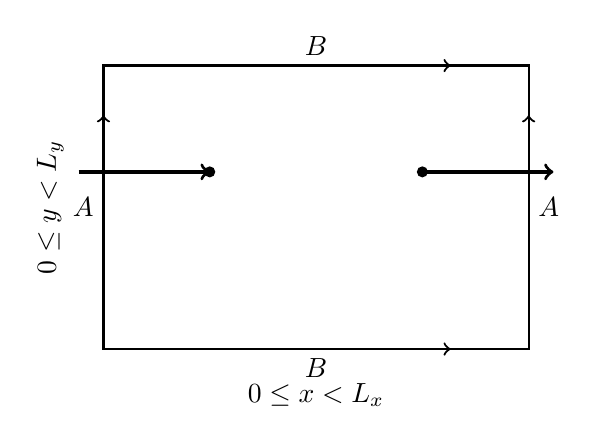
\begin{tikzpicture}[x=0.9cm,y=0.9cm]
\draw[thick] (0,0) rectangle (6,4);
\draw[->,thick] (0,0.7) -- (0,3.3);
\draw[->,thick] (6,0.7) -- (6,3.3);
\draw[->,thick] (1.1,0) -- (4.9,0);
\draw[->,thick] (1.1,4) -- (4.9,4);
\node[left] at (0,2) {$A$};
\node[right] at (6,2) {$A$};
\node[below] at (3,0) {$B$};
\node[above] at (3,4) {$B$};
\draw[->,very thick] (4.5,2.5) -- (6.35,2.5);
\draw[->,very thick] (-0.35,2.5) -- (1.5,2.5);
\fill (4.5,2.5) circle (2pt);
\fill (1.5,2.5) circle (2pt);
\node at (3,-0.65) {$0\leq x<L_x$};
\node[rotate=90] at (-0.75,2) {$0\leq y<L_y$};
\end{tikzpicture}
\caption{二维周期空间：带有相同标记的边被等同，因此穿过一条边的粒子会在对边对应点重新出现。}
\end{figure}

\begin{classroomqa}
\lecturetimestamp{01:50:58}
\audiencequestion{周期构造表示的是空间，还是空间中的物体？}
\lecturerresponse{它表示空间。物体和场生活在该空间中，并遵守其等同关系。引入周期性是为了控制无限体积问题；通过取体积很大并将动量求和替换为积分，可以将其去除。}
\end{classroomqa}

三维类比是一个立方体，其中三对相对的面被等同。左面和右面相同，上面和下面相同，前面和后面相同。穿过任何一个面的粒子都会通过其等同伙伴重新出现。\footnote{周期立方体及其三对等同面见01：51：27--01：52：17。\(k_i\)的显示方程是先前条件\(kL=2\pi n\)的分量式重构，应用于三个周期方向。}三个动量分量满足
\begin{equation}
k_i=\frac{2\pi n_i}{L_i},
\qquad i=x,y,z,
\end{equation}
每个方向有一个整数\(n_i\)。环面可以按同样的规则定义在任意维数中。

\begin{figure}[t]
\centering
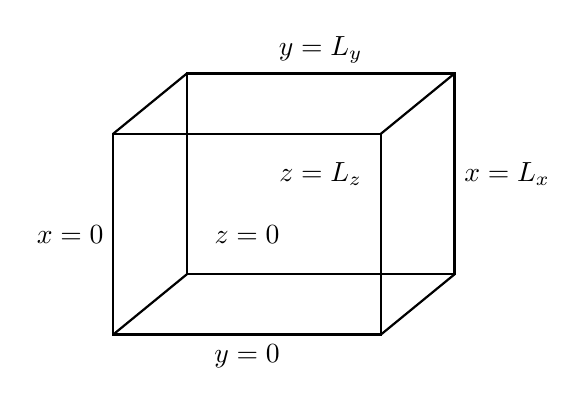
\begin{tikzpicture}[scale=0.85]
\draw[thick] (0,0) rectangle (4,3);
\draw[thick] (1.1,0.9) rectangle (5.1,3.9);
\draw[thick] (0,0) -- (1.1,0.9);
\draw[thick] (4,0) -- (5.1,0.9);
\draw[thick] (4,3) -- (5.1,3.9);
\draw[thick] (0,3) -- (1.1,3.9);
\node[left] at (0,1.5) {$x=0$};
\node[right] at (5.1,2.4) {$x=L_x$};
\node[below] at (2,0) {$y=0$};
\node[above] at (3.1,3.9) {$y=L_y$};
\node at (2,1.5) {$z=0$};
\node at (3.1,2.4) {$z=L_z$};
\end{tikzpicture}
\caption{三维周期空间，表现为每对相对的面都被等同的立方体。}
\end{figure}

\begin{classroomqa}
\lecturetimestamp{01:52:20}
\audiencequestion{场论会为空间选择一个物理的网格大小吗？}
\lecturerresponse{这是一个推测性问题。就这里的实际目的而言，空间是连续的。量子是粒子，而不是空间网格的单元。在圆周构造中，变得离散的是动量；位置仍然是连续且周期的。}
\end{classroomqa}

\editorialnote{在关于网格大小的交流中，有一段很长的损坏段落提到了普朗克尺度，但没有保留任何关于基本空间离散性的可恢复主张。这里不推断此类主张。}

\(k\)的离散性完全来自施加周期波函数。这并不证明坐标\(x\)本身位于点阵上。质疑空间是否可能具有基本微观结构是合理的，但这是一个独立的、推测性的问题。

\section{费米子与外部场}

玻色模式允许任意非负占据数。费米子要求相反的行为：泡利不相容原理禁止两个全同费米子占据同一状态。

\begin{classroomqa}
\lecturetimestamp{01:55:13}
\audiencequestion{把对易子替换为反对易子，会给出最简单的费米子理论吗？}
\lecturerresponse{本质上是的。对易子是\([A,B]=AB-BA\)，而反对易子是\(\{A,B\}=AB+BA\)。相应的费米子产生与湮灭代数实现了泡利不相容：第二个全同费米子不能被放入已被占据的状态。详细理论留待后述。}
\end{classroomqa}

两个乘积相差一个符号：
\begin{equation}
[A,B]=AB-BA,
\qquad
\{A,B\}=AB+BA.
\end{equation}
对易子在交换下是反对称的，而反对易子是对称的。若一个反对易子为零，则
\begin{equation}
\{A,B\}=0
\quad\Longrightarrow\quad
AB=-BA.
\end{equation}
对于这样一对算符，交换两个费米子算符会改变符号。这比普通的可交换情形更不寻常，在普通可交换情形中\([A,B]=0\)给出\(AB=BA\)。把玻色对易子替换为相应的反对易代数，是导致费米子的数学改变；其详细展开留待后述。

反对易关系逆转了玻色子所呈现的统计行为。不存在全同费米子在同一模式中的受激堆积；该模式的占据会阻止另一个全同费米子进入其中。由于单个费米子态至多只能容纳一个全同费米子，因此把任意大量全同费米子放入该单一态并不能得到经典场极限。

\begin{classroomqa}
\lecturetimestamp{01:58:03}
\audiencequestion{{\proseunicodefont α}粒子由费米子组成，怎么可能是玻色子？}
\lecturerresponse{含有偶数个费米子组分的束缚复合体可以具有玻色统计。把若干个这样的复合玻色子放入同一个整体态，并不等同于把它们的各个费米子组分放入同一个全同单粒子态。}
\end{classroomqa}

复合粒子的统计性质关注的是作为整体的束缚客体。因此，费米子组分可以结合成一个表现为玻色子的客体，而不违反组分所服从的泡利不相容原理。

\begin{classroomqa}
\lecturetimestamp{01:58:33}
\audiencequestion{外部场如何纳入？}
\lecturerresponse{到目前为止的构造中尚未包含任何外部背景场。这样的场可以作为经典场给定，也可以用包含大量量子的态在量子力学上表示。}
\end{classroomqa}

要使这两种描述一致，大占据态必须被适当制备并且相位相干；仅靠粒子数并不足够。\footnote{交换提供了多量子尺度。这里把相位相干表述为防止仅凭大占据就被误认为经典场的附加条件。} 在该半经典区域中，二者的效应在微小量子偏差范围内一致。这是一个基本的一致性条件。当单个量子起作用时，电磁场必须描述离散的光子；然而，一个适当相位相干且包含大量光子的态必须重现经典电磁波的熟悉作用。
